%*************
%preamble
%*************
	\documentclass[notitlepage,a4paper]{article}

%**********
%packages
%**********
	\usepackage[english]{babel}%required allways
	\usepackage{booktabs}	%required for bookstyle tables, without these the tables will have to be redraw

	\usepackage{tikz}		% required for linestyle graphics
	\usetikzlibrary{patterns}% required for fill styles
	\usepgfmodule{plot}		% for plots of functions

	\usepackage{float} 		% required for example and excercise styles

	\usepackage[intlimits]{amsmath}%provide option intlimits to
				% give boundaries of limits above/below integral sign
	\usepackage{rotating} 	%required for rotated tables
	\usepackage{graphicx} 	%required for including external graphics files
	\usepackage{caption}
	\usepackage[official]{eurosym}

%*************
%declarations
%*************
	\setlength{\topmargin}{0in}
	\setlength{\textheight}{641pt}
	\setlength{\oddsidemargin}{11pt}
	\setlength{\evensidemargin}{11pt}
	\setlength{\textwidth}{431pt}

\begin{document}
	\date{ 8-06-2012}
	\title{classLatex Help file}
	\author{Louis Chaillet}

\section*{classLatex tabel command in OX}
Latex::table( ...)
	expects any of the following pairs of variables in any order:
\begin{itemize}
\item 		"\%h", string, goes above the table centered across columns;
\item		"\%hc", integer, count of header rows, default is 1;
\item		"\%r", array of string, rowheaders last one should be for the total;
\item		"\%c", array of string, column headers;
\item		"\%b", matrix of body (the numbers);
\item		"\%t", matrix of totals;
\item		"\%l", string with the caption, default none;
\item		"\%i", enumerated, class supplied, (latex.above or latex.below), caption position can be above or below, default is below;
\item		"\%f", string with number format to use in the table, default variable ox format;
\item		"\%x", string for reference, default none;
\item		"\%e", string extra after bottomrule but within tabular, default none;
\item		"\%lo", integer, value 1 results in lower diagonal print only, useful for correlation matrix, default zero will print full table matrix;
\item		"\%sz", string, will suppress zeros in the table in favor of this string, default none, zeros will show;
\item		"\%ro", integer, value 1 rotates table counterclockwise 90 degrees, default not rotated;
\item		"\%td", string with latex table definition, the columns you want, defaults to a useful set.
\end{itemize}

Example latex output from OX.
\begin{verbatim}
\begin{table}[!h]
    \centering
    \caption*{Compiled pdf table from latex}
    \begin{tabular}{l r r r r }
         \toprule
         & Beta & Premium & EFM  & Volatility\\
         &  &  & view & \\
         Factor &  & (\%)& (\%) & (\%)\\
         \midrule
         F1: EPRA Europe &   1.00 	&  4.37 &  	& 16.10\\
         F2: MSCI USA 	 &	 0		&	3.8 &	& 17.00 \\
         \bottomrule
     \end{tabular}
\end{table}
\end{verbatim}

\begin{table}[!h]
	\centering
	\caption*{Compiled pdf table from latex}
	\begin{tabular}{l r r r r }
		\toprule
		 & Beta & Premium & EFM  & Volatility\\
		  &  &  & view & \\
		 Factor &  & (\%)$^\dagger$ & (\%)$^\ddag$ & (\%)\\
		 		\midrule
		F1: EPRA Europe &   1.00 	&  4.37 	&  & 16.10\\
        F2: MSCI USA 	 &	 0		&	3.8 	&  & 17.00 \\
         \bottomrule
	\end{tabular}
\end{table}


\clearpage
\section*{classLatex cfdist command in OX}
Latex::cfdist ( ...)
	expects any of the following pairs of variables:
\begin{itemize}
\item		"\%pd", matrix with percentile distributions to show;
\item		"\%mm", matrix with exact means, default is calculated means;
\item		"\%b", matrix of body (the numbers) the distribution to show in this case;
\item		"\%xv", vector of xlabels, defaults to year 1, 2 etc;
\item		"\%h", string, goes above the table centered across columns;
\item		"\%l", string with the caption;
\item		"\%f", string with number format, default is set to 1 decimal;
\item		"\%x", string for reference;
\item		"\%i", latex.above or latex.below, caption position above or below, defaults to below;
\item		"\%dt", double, thickness of the bar, default 1 is sensible;
\item		"\%dl", double, position from the left textmargin, default 0.1 is sensible;
\item		"\%rc", string, right color in shade, default white;
\item		"\%lc", string, left color in shade, default red;
\item		"\%o", binary, include one point no or yes, default is yes;
\item		"\%c", string to name the distribution;
\item		"\%w", double, width of bars, default is 0.5, this works well;
\item		"\%n", text width node to place in graph*/
\end{itemize}


Example latex output from OX.
\begin{verbatim}
\begin{figure}[h!]
\centering
    \caption*{Compiled pdf (tikz) graph from latex}
    \begin{minipage}[c]{1\textwidth} The mean cash flows (black solid lines)
    are calibrated to the projected cash flows (values shown). The box plots
    summarize the probability distribution (assumed to be lognormal): the bottom
    and top of the box are the 10$^\textrm{th}$ and 90$^\textrm{th}$ percentile,
    and the red dashed horizontal line is the median. 	 \end{minipage}
    \begin{tikzpicture}[terminal/.style={
        thick, draw=black,
        rectangle,minimum size=6mm,rounded corners=3mm,
        top color=white, bottom color=white}]
        %y-axes
        \draw[->,color=black] (0 ,-0.01\textwidth) --
        (0, 0.524427\textwidth) node [above] {$CF$};
        %y-axis ticks
        \foreach \y/\ytext in
        {0/0,0.0824045/100,0.164809/200,0.247214/300,
            0.329618/400,0.412023/500,0.494427/600}
        \draw[yshift=\y \textwidth] (0pt,0pt) --
           (-3pt,0pt) node[left,fill=white] {$\ytext$};
        %bars

   Commands omitted here for brevity ....

        %bars
        %mean
        \draw[color = black, thick] (0.025000\textwidth-0.01,0.000000\textwidth )
            -- (0.075000\textwidth+0.01,0.000000\textwidth) node [terminal, above] {0};
        %median
        \draw[color = red, dashed, thick] (0.025000\textwidth-0.01,0.000000\textwidth)
            -- (0.075000\textwidth+0.01,0.000000\textwidth) ;
        %scale point
        \draw[thin, color = black] (0.05\textwidth, 0) --
           (0.05\textwidth, -0.01\textwidth)
           node [anchor=north east, rotate=45] {2013/6};
        %x-axes
        \draw[color=black, thin] (0.81\textwidth, 0) -- (0,0);
        \node at (0,-0.01\textwidth) [anchor = north east,rotate = 45] {Y/M};
        \node at (0.2\textwidth, 0.4\textwidth)[terminal]{NAV 150.00; IRR 15.05};
    \end{tikzpicture}
\end{figure}
\end{verbatim}

\begin{figure}[h!]
\centering
	\caption*{Compiled pdf (tikz) graph from \LaTeX}
	\begin{minipage}[c]{1\textwidth} The mean cash flows (black solid lines) are calibrated to the projected cash flows (values shown). The box plots summarize the probability distribution (assumed to be lognormal): the bottom and top of the box are the 10$^\textrm{th}$ and 90$^\textrm{th}$ percentile, and the red dashed horizontal line is the median. 	 \end{minipage}
	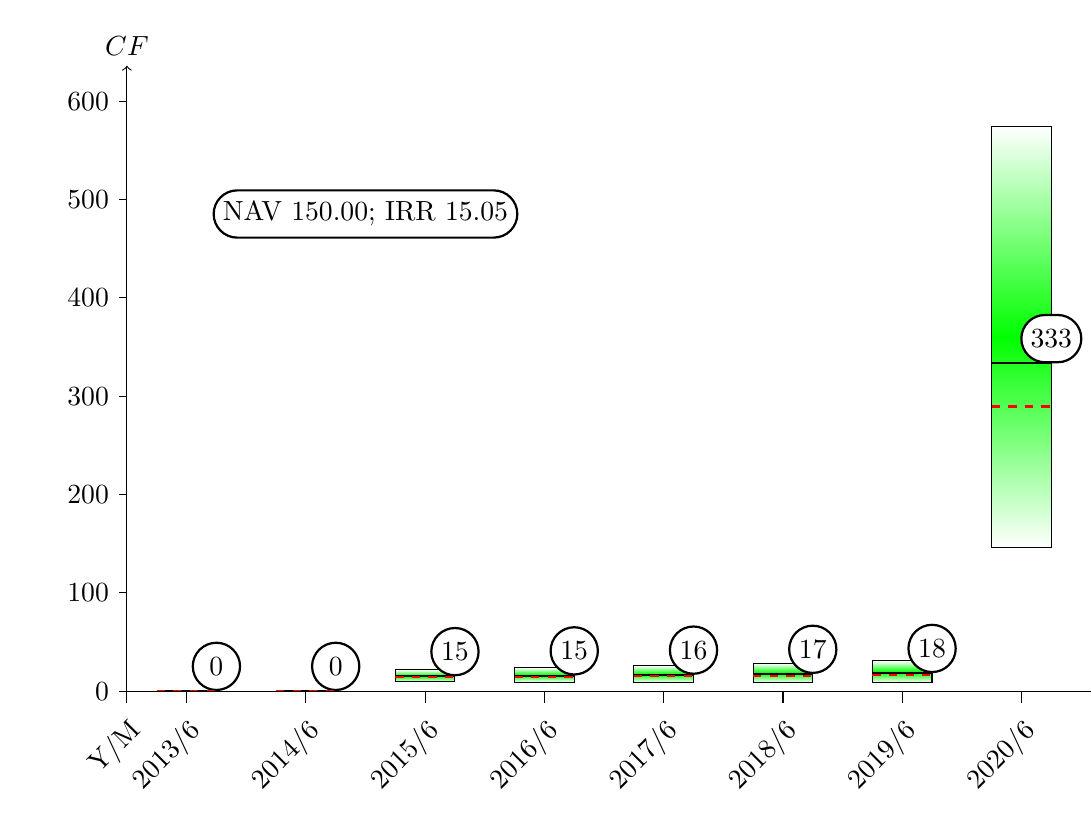
\begin{tikzpicture}[terminal/.style={
		thick, draw=black,
		rectangle,minimum size=6mm,rounded corners=3mm,
		top color=white, bottom color=white}]
		%y-axes
		\draw[->,color=black] (0 ,-0.01\textwidth) --
		(0, 0.524427\textwidth) node [above] {$CF$};
		%y-axis ticks
		\foreach \y/\ytext in {0/0,0.0824045/100,0.164809/200,0.247214/300,0.329618/400,0.412023/500,0.494427/600}
 		\draw[yshift=\y \textwidth] (0pt,0pt) -- (-3pt,0pt) node[left,fill=white] {$\ytext$};
		%bars
		\shadedraw[bottom color=white, top color=white, middle color=green] (0.725000\textwidth, 0.120301\textwidth)
			--(0.725000\textwidth, 0.473411\textwidth)
			--(0.775000\textwidth, 0.473411\textwidth)
			--(0.775000\textwidth, 0.120301\textwidth)
			-- cycle;
		%mean
		\draw[color = black, thick] (0.725000\textwidth-0.01,0.274785\textwidth )
			 -- (0.775000\textwidth+0.01,0.274785\textwidth) node [terminal, above] {333};
		%median
		\draw[color = red, dashed, thick] (0.725000\textwidth-0.01,0.238646\textwidth )
			 -- (0.775000\textwidth+0.01,0.238646\textwidth) ;
		%scale point
		\draw[thin, color = black] (0.75\textwidth, 0) -- (0.75\textwidth, -0.01\textwidth)
		 node [anchor=north east, rotate=45] {2020/6};
		%bars
		\shadedraw[bottom color=white, top color=white, middle color=green] (0.625000\textwidth, 0.006964\textwidth)
			--(0.625000\textwidth, 0.025329\textwidth)
			--(0.675000\textwidth, 0.025329\textwidth)
			--(0.675000\textwidth, 0.006964\textwidth)
			-- cycle;
		%mean
		\draw[color = black, thick] (0.625000\textwidth-0.01,0.015024\textwidth )
			 -- (0.675000\textwidth+0.01,0.015024\textwidth) node [terminal, above] {18};
		%median
		\draw[color = red, dashed, thick] (0.625000\textwidth-0.01,0.013281\textwidth )
			 -- (0.675000\textwidth+0.01,0.013281\textwidth) ;
		%scale point
		\draw[thin, color = black] (0.65\textwidth, 0) -- (0.65\textwidth, -0.01\textwidth)
		 node [anchor=north east, rotate=45] {2019/6};
		%bars
		\shadedraw[bottom color=white, top color=white, middle color=green] (0.525000\textwidth, 0.007117\textwidth)
			--(0.525000\textwidth, 0.023284\textwidth)
			--(0.575000\textwidth, 0.023284\textwidth)
			--(0.575000\textwidth, 0.007117\textwidth)
			-- cycle;
		%mean
		\draw[color = black, thick] (0.525000\textwidth-0.01,0.014309\textwidth )
			 -- (0.575000\textwidth+0.01,0.014309\textwidth) node [terminal, above] {17};
		%median
		\draw[color = red, dashed, thick] (0.525000\textwidth-0.01,0.012873\textwidth )
			 -- (0.575000\textwidth+0.01,0.012873\textwidth) ;
		%scale point
		\draw[thin, color = black] (0.55\textwidth, 0) -- (0.55\textwidth, -0.01\textwidth)
		 node [anchor=north east, rotate=45] {2018/6};
		%bars
		\shadedraw[bottom color=white, top color=white, middle color=green] (0.425000\textwidth, 0.007310\textwidth)
			--(0.425000\textwidth, 0.021299\textwidth)
			--(0.475000\textwidth, 0.021299\textwidth)
			--(0.475000\textwidth, 0.007310\textwidth)
			-- cycle;
		%mean
		\draw[color = black, thick] (0.425000\textwidth-0.01,0.013628\textwidth )
			 -- (0.475000\textwidth+0.01,0.013628\textwidth) node [terminal, above] {16};
		%median
		\draw[color = red, dashed, thick] (0.425000\textwidth-0.01,0.012478\textwidth )
			 -- (0.475000\textwidth+0.01,0.012478\textwidth) ;
		%scale point
		\draw[thin, color = black] (0.45\textwidth, 0) -- (0.45\textwidth, -0.01\textwidth)
		 node [anchor=north east, rotate=45] {2017/6};
		%bars
		\shadedraw[bottom color=white, top color=white, middle color=green] (0.325000\textwidth, 0.007504\textwidth)
			--(0.325000\textwidth, 0.019495\textwidth)
			--(0.375000\textwidth, 0.019495\textwidth)
			--(0.375000\textwidth, 0.007504\textwidth)
			-- cycle;
		%mean
		\draw[color = black, thick] (0.325000\textwidth-0.01,0.012979\textwidth )
			 -- (0.375000\textwidth+0.01,0.012979\textwidth) node [terminal, above] {15};
		%median
		\draw[color = red, dashed, thick] (0.325000\textwidth-0.01,0.012095\textwidth )
			 -- (0.375000\textwidth+0.01,0.012095\textwidth) ;
		%scale point
		\draw[thin, color = black] (0.35\textwidth, 0) -- (0.35\textwidth, -0.01\textwidth)
		 node [anchor=north east, rotate=45] {2016/6};
		%bars
		\shadedraw[bottom color=white, top color=white, middle color=green] (0.225000\textwidth, 0.007700\textwidth)
			--(0.225000\textwidth, 0.017852\textwidth)
			--(0.275000\textwidth, 0.017852\textwidth)
			--(0.275000\textwidth, 0.007700\textwidth)
			-- cycle;
		%mean
		\draw[color = black, thick] (0.225000\textwidth-0.01,0.012361\textwidth )
			 -- (0.275000\textwidth+0.01,0.012361\textwidth) node [terminal, above] {15};
		%median
		\draw[color = red, dashed, thick] (0.225000\textwidth-0.01,0.011724\textwidth )
			 -- (0.275000\textwidth+0.01,0.011724\textwidth) ;
		%scale point
		\draw[thin, color = black] (0.25\textwidth, 0) -- (0.25\textwidth, -0.01\textwidth)
		 node [anchor=north east, rotate=45] {2015/6};
		%bars
		%mean
		\draw[color = black, thick] (0.125000\textwidth-0.01,0.000000\textwidth )
			 -- (0.175000\textwidth+0.01,0.000000\textwidth) node [terminal, above] {0};
		%median
		\draw[color = red, dashed, thick] (0.125000\textwidth-0.01,0.000000\textwidth )
			 -- (0.175000\textwidth+0.01,0.000000\textwidth) ;
		%scale point
		\draw[thin, color = black] (0.15\textwidth, 0) -- (0.15\textwidth, -0.01\textwidth)
		 node [anchor=north east, rotate=45] {2014/6};
		%bars
		%mean
		\draw[color = black, thick] (0.025000\textwidth-0.01,0.000000\textwidth )
			 -- (0.075000\textwidth+0.01,0.000000\textwidth) node [terminal, above] {0};
		%median
		\draw[color = red, dashed, thick] (0.025000\textwidth-0.01,0.000000\textwidth )
			 -- (0.075000\textwidth+0.01,0.000000\textwidth) ;
		%scale point
		\draw[thin, color = black] (0.05\textwidth, 0) -- (0.05\textwidth, -0.01\textwidth)
		 node [anchor=north east, rotate=45] {2013/6};
		%x-axes
		\draw[color=black, thin] (0.81\textwidth, 0) -- (0,0);
		\node at (0,-0.01\textwidth) [anchor = north east,rotate = 45] {Y/M};
		\node at (0.2\textwidth, 0.4\textwidth)[terminal]{NAV 150.00; IRR 15.05};
	\end{tikzpicture}
\end{figure}

	\clearpage

\section*{classLatex distbar command in OX}

Example latex output from OX.
\begin{verbatim}
\begin{figure}[h!]
\centering
    \caption*{Example compiled distbar in pdf}
    \begin{minipage}[c]{1\textwidth} The graph below gives a distribution
    of the money returned form the investment project. The vertical line
    marked with 'one time' is the point in the distribution where the money
    is returned exactly one time. 	 \end{minipage}
    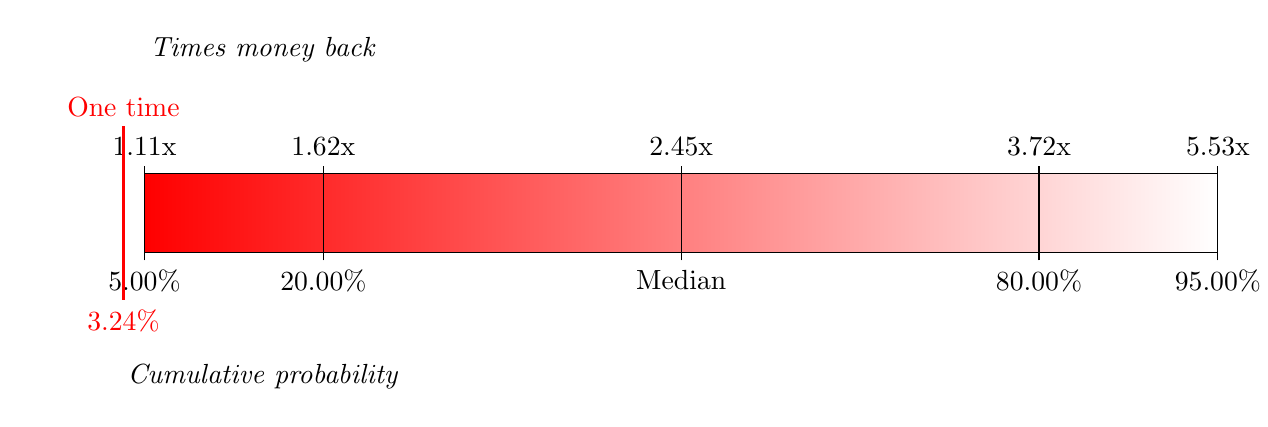
\begin{tikzpicture}
        %labels
        \node at(0.2*\textwidth,-1.3) [below ]{\emph{Cumulative probability}};
        \node at(0.2*\textwidth,2.3) [above ]{\emph{Times money back}};
        \%bar
        \shadedraw[left color=red, right color=white] (0.1*\textwidth,0)
            -- (1*\textwidth,0)
            -- (1*\textwidth,1)
            -- (0.1*\textwidth,1)
            -- cycle;
        %  5.00\%
        \draw (0.1*\textwidth, -0.1) node [below]{  5.00\%} --
        (0.1*\textwidth, 1.1) node [above] {  1.11x};
        % 20.00\%
        \draw (0.25*\textwidth, -0.1) node [below]{ 20.00\%} --
        (0.25*\textwidth, 1.1) node [above] {  1.62x};
        %Median
        \draw (0.55*\textwidth, -0.1) node [below]{Median} --
            (0.55*\textwidth, 1.1) node [above] {  2.45x};
        % 80.00\%
        \draw (0.85*\textwidth, -0.1) node [below]{ 80.00\%} --
            (0.85*\textwidth, 1.1) node [above] {  3.72x};
        % 95.00\%
        \draw (1*\textwidth, -0.1) node [below]{ 95.00\%} -- (1*\textwidth, 1.1) node [above] {  5.53x};
        %1 time
        \draw [thick,red](0.0824*\textwidth,-0.6) node [below]{3.24\%}
            -- (0.0824*\textwidth, 1.6) node [above]{One time} ;
    \end{tikzpicture}
\end{figure}
\end{verbatim}

\begin{figure}[h!]
\centering
	\caption*{Example compiled distbar in pdf}
	\begin{minipage}[c]{1\textwidth} The graph below gives a distribution of the money returned form the investment project. The vertical line marked with 'one time' is the point in the distribution where the money is returned exactly one time. 	 \end{minipage}
	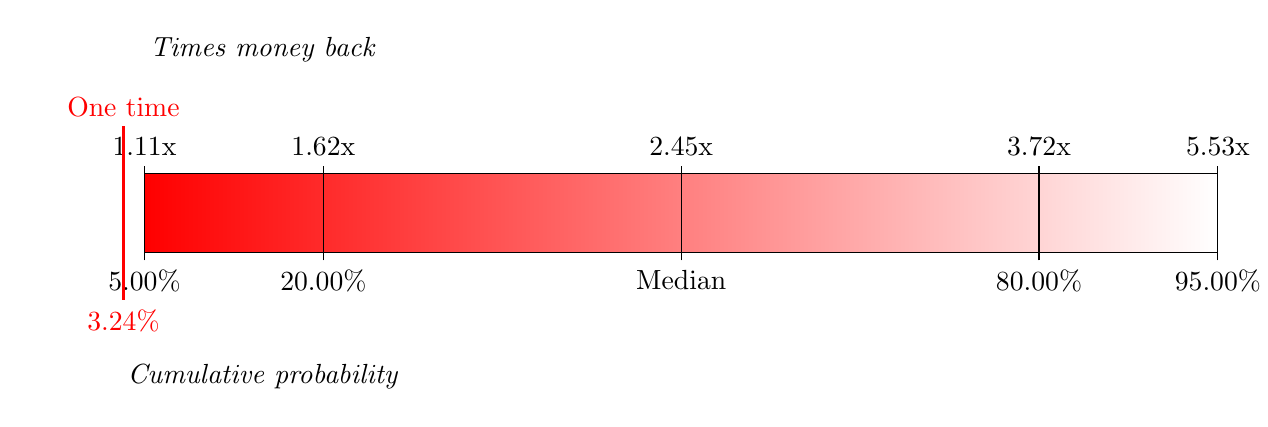
\begin{tikzpicture}
		%labels
		\node at(0.2*\textwidth,-1.3) [below ]{\emph{Cumulative probability}};
		\node at(0.2*\textwidth,2.3) [above ]{\emph{Times money back}};
		\%bar
		\shadedraw[left color=red, right color=white] (0.1*\textwidth,0)
			-- (1*\textwidth,0)
			-- (1*\textwidth,1)
			-- (0.1*\textwidth,1)
			-- cycle;
		%  5.00\%
		\draw (0.1*\textwidth, -0.1) node [below]{  5.00\%} -- (0.1*\textwidth, 1.1) node [above] {  1.11x};
		% 20.00\%
		\draw (0.25*\textwidth, -0.1) node [below]{ 20.00\%} -- (0.25*\textwidth, 1.1) node [above] {  1.62x};
		%Median
		\draw (0.55*\textwidth, -0.1) node [below]{Median} -- (0.55*\textwidth, 1.1) node [above] {  2.45x};
		% 80.00\%
		\draw (0.85*\textwidth, -0.1) node [below]{ 80.00\%} -- (0.85*\textwidth, 1.1) node [above] {  3.72x};
		% 95.00\%
		\draw (1*\textwidth, -0.1) node [below]{ 95.00\%} -- (1*\textwidth, 1.1) node [above] {  5.53x};
		%1 time
		\draw [thick,red](0.0824*\textwidth,-0.6) node [below]{3.24\%}
			-- (0.0824*\textwidth, 1.6) node [above]{One time} ;
	\end{tikzpicture}
\end{figure}

\clearpage
\section*{classLatex density command in OX}

Example latex density output from OX.
\begin{verbatim}
\begin{figure}[h!]
\centering
    \caption*{\textbf{Model output: distribution of the internal rate of return}}
    \begin{tikzpicture}
    %x-axes
    \draw[->,color=black, thin] (-0.129584\textwidth, 0) --
        (0.710416\textwidth,0) node [right] {$x$} ;
    %x-axis ticks
    \foreach \x/\xtext in {-0.119584/-20\%, 0.013750/-10\%, 0.147083/0\%, 0.280416/10\%,
        0.413750/20\%, 0.547083/30\%, 0.680416/40\%}
        \draw[xshift=\x \textwidth] (0pt,0pt) -- (0pt,-3pt) node[below] {$\xtext$};
    %y-axes
    \draw[->,color=black, thin](-0.119584\textwidth ,-0.01\textwidth) --
        (-0.119584\textwidth, 0.524427\textwidth) node[above] {$p(x)$};
    %y-axis ticks
    \foreach \y/\ytext in {0.000000/  0.00,0.123607/  0.10,0.247214/  0.20,
        0.370820/  0.30,0.494427/  0.40}
        \draw[yshift=\y \textwidth] (-0.119584\textwidth, 0pt) --
            (-0.119584\textwidth -3pt,0pt) node[left] {$\ytext$};
    %density lines
    \draw  [red, thick] plot [smooth] coordinates {
        (0.000000\textwidth,0.002674\textwidth)
        (0.005820\textwidth,0.003313\textwidth)

Command ommited for brevity ...

        (0.570380\textwidth,0.031912\textwidth)
        (0.576200\textwidth,0.027252\textwidth)
    };
    \end{tikzpicture}
\end{figure}
\end{verbatim}

\begin{figure}[h!]
\centering
	\caption*{\textbf{Model output: distribution of the internal rate of return}}
	\begin{tikzpicture}
	%x-axes
	\draw[->,color=black, thin] (-0.129584\textwidth, 0) --
		(0.710416\textwidth,0) node [right] {$x$} ;
	%x-axis ticks
	\foreach \x/\xtext in {-0.119584/-20\%, 0.013750/-10\%, 0.147083/0\%, 0.280416/10\%, 0.413750/20\%, 0.547083/30\%, 0.680416/40\%}
 		\draw[xshift=\x \textwidth] (0pt,0pt) -- (0pt,-3pt) node[below] {$\xtext$};
	%y-axes
	\draw[->,color=black, thin](-0.119584\textwidth ,-0.01\textwidth) --
		(-0.119584\textwidth, 0.524427\textwidth) node[above] {$p(x)$};
	%y-axis ticks
	\foreach \y/\ytext in {0.000000/  0.00,0.123607/  0.10,0.247214/  0.20,0.370820/  0.30,0.494427/  0.40}
 		\draw[yshift=\y \textwidth] (-0.119584\textwidth, 0pt) -- (-0.119584\textwidth -3pt,0pt) node[left] {$\ytext$};
	%density lines
	\draw  [red, thick] plot [smooth] coordinates {
		(0.000000\textwidth,0.002674\textwidth)
		(0.005820\textwidth,0.003313\textwidth)
		(0.011640\textwidth,0.004071\textwidth)
		(0.017461\textwidth,0.004966\textwidth)
		(0.023281\textwidth,0.006013\textwidth)
		(0.029101\textwidth,0.007232\textwidth)
		(0.034921\textwidth,0.008643\textwidth)
		(0.040741\textwidth,0.010267\textwidth)
		(0.046562\textwidth,0.012128\textwidth)
		(0.052382\textwidth,0.014254\textwidth)
		(0.058202\textwidth,0.016673\textwidth)
		(0.064022\textwidth,0.019416\textwidth)
		(0.069842\textwidth,0.022520\textwidth)
		(0.075663\textwidth,0.026020\textwidth)
		(0.081483\textwidth,0.029956\textwidth)
		(0.087303\textwidth,0.034368\textwidth)
		(0.093123\textwidth,0.039297\textwidth)
		(0.098943\textwidth,0.044782\textwidth)
		(0.104764\textwidth,0.050862\textwidth)
		(0.110584\textwidth,0.057570\textwidth)
		(0.116404\textwidth,0.064935\textwidth)
		(0.122224\textwidth,0.072984\textwidth)
		(0.128044\textwidth,0.081733\textwidth)
		(0.133865\textwidth,0.091195\textwidth)
		(0.139685\textwidth,0.101373\textwidth)
		(0.145505\textwidth,0.112262\textwidth)
		(0.151325\textwidth,0.123849\textwidth)
		(0.157145\textwidth,0.136112\textwidth)
		(0.162966\textwidth,0.149019\textwidth)
		(0.168786\textwidth,0.162529\textwidth)
		(0.174606\textwidth,0.176590\textwidth)
		(0.180426\textwidth,0.191140\textwidth)
		(0.186246\textwidth,0.206109\textwidth)
		(0.192067\textwidth,0.221413\textwidth)
		(0.197887\textwidth,0.236963\textwidth)
		(0.203707\textwidth,0.252657\textwidth)
		(0.209527\textwidth,0.268390\textwidth)
		(0.215347\textwidth,0.284048\textwidth)
		(0.221168\textwidth,0.299516\textwidth)
		(0.226988\textwidth,0.314678\textwidth)
		(0.232808\textwidth,0.329423\textwidth)
		(0.238628\textwidth,0.343644\textwidth)
		(0.244448\textwidth,0.357244\textwidth)
		(0.250269\textwidth,0.370134\textwidth)
		(0.256089\textwidth,0.382238\textwidth)
		(0.261909\textwidth,0.393490\textwidth)
		(0.267729\textwidth,0.403829\textwidth)
		(0.273549\textwidth,0.413203\textwidth)
		(0.279370\textwidth,0.421561\textwidth)
		(0.285190\textwidth,0.428852\textwidth)
		(0.291010\textwidth,0.435026\textwidth)
		(0.296830\textwidth,0.440032\textwidth)
		(0.302650\textwidth,0.443822\textwidth)
		(0.308471\textwidth,0.446354\textwidth)
		(0.314291\textwidth,0.447596\textwidth)
		(0.320111\textwidth,0.447534\textwidth)
		(0.325931\textwidth,0.446170\textwidth)
		(0.331751\textwidth,0.443527\textwidth)
		(0.337572\textwidth,0.439650\textwidth)
		(0.343392\textwidth,0.434600\textwidth)
		(0.349212\textwidth,0.428452\textwidth)
		(0.355032\textwidth,0.421290\textwidth)
		(0.360852\textwidth,0.413199\textwidth)
		(0.366673\textwidth,0.404263\textwidth)
		(0.372493\textwidth,0.394558\textwidth)
		(0.378313\textwidth,0.384155\textwidth)
		(0.384133\textwidth,0.373115\textwidth)
		(0.389953\textwidth,0.361497\textwidth)
		(0.395774\textwidth,0.349355\textwidth)
		(0.401594\textwidth,0.336748\textwidth)
		(0.407414\textwidth,0.323735\textwidth)
		(0.413234\textwidth,0.310384\textwidth)
		(0.419054\textwidth,0.296769\textwidth)
		(0.424875\textwidth,0.282967\textwidth)
		(0.430695\textwidth,0.269064\textwidth)
		(0.436515\textwidth,0.255141\textwidth)
		(0.442335\textwidth,0.241282\textwidth)
		(0.448155\textwidth,0.227565\textwidth)
		(0.453976\textwidth,0.214062\textwidth)
		(0.459796\textwidth,0.200836\textwidth)
		(0.465616\textwidth,0.187944\textwidth)
		(0.471436\textwidth,0.175432\textwidth)
		(0.477256\textwidth,0.163338\textwidth)
		(0.483077\textwidth,0.151692\textwidth)
		(0.488897\textwidth,0.140515\textwidth)
		(0.494717\textwidth,0.129820\textwidth)
		(0.500537\textwidth,0.119615\textwidth)
		(0.506357\textwidth,0.109897\textwidth)
		(0.512178\textwidth,0.100661\textwidth)
		(0.517998\textwidth,0.091895\textwidth)
		(0.523818\textwidth,0.083584\textwidth)
		(0.529638\textwidth,0.075712\textwidth)
		(0.535458\textwidth,0.068262\textwidth)
		(0.541279\textwidth,0.061219\textwidth)
		(0.547099\textwidth,0.054573\textwidth)
		(0.552919\textwidth,0.048319\textwidth)
		(0.558739\textwidth,0.042454\textwidth)
		(0.564559\textwidth,0.036983\textwidth)
		(0.570380\textwidth,0.031912\textwidth)
		(0.576200\textwidth,0.027252\textwidth)
	};
	\end{tikzpicture}
\end{figure}

\end{document}
